\documentclass[10pt]{oblivoir}

% ---------------------------------------------- PACKAGE IMPORTS
\usepackage{kotex}
\usepackage{amsmath}
\usepackage{multicol}
\usepackage{fixltx2e}
\usepackage{float}
\usepackage{graphicx}
\usepackage{fullpage}
\usepackage{siunitx}
\usepackage[ruled,vlined]{algorithm2e}
\usepackage{hyperref}
\usepackage{listings}
\usepackage{color}
\usepackage{caption}
\usepackage{indentfirst}
\usepackage{subcaption}
\usepackage{tikz-cd}
\usepackage{chngcntr}
\usepackage{comment}
\usepackage[nameinlink]{cleveref}

% ---------------------------------------------- FIGURE COUNTER SETTINGS
% \counterwithin{figure}{section}

% ---------------------------------------------- CODE AREA SETTINGS
\definecolor{dkgreen}{rgb}{0,0.6,0}
\definecolor{gray}{rgb}{0.5,0.5,0.5}
\definecolor{mauve}{rgb}{0.58,0,0.82}

\lstset{frame=tb,
  language=C++,
  aboveskip=3mm,
  belowskip=3mm,
  showstringspaces=false,
  columns=flexible,
  basicstyle={\small\ttfamily},
  numbers=none,
  numberstyle=\tiny\color{gray},
  keywordstyle=\color{blue},
  commentstyle=\color{dkgreen},
  stringstyle=\color{mauve},
  breaklines=true,
  breakatwhitespace=true,
  tabsize=3
}

% ---------------------------------------------- CLEVERREF SETTINGS
\crefname{figure}{그림}{그림}
\crefname{equation}{식}{식}
\crefname{table}{표}{표}
\crefname{listing}{목록}{목록}
\crefname{section}{절}{절}
\crefname{algorithm}{알고리즘}{알고리즘}

\captionsetup[subfigure]{subrefformat=simple,labelformat=simple}
    \renewcommand\thesubfigure{ (\alph{subfigure})}

% ---------------------------------------------- GENERAL SETTINGS
\setlength{\parindent}{0.3cm} % The first indent width setup

% ---------------------------------------------- CUSTOM COMMANDS
%       GENERAL
\newcommand{\textss}[1]{\scriptsize#1\normalsize}
%       MATHEMATICAL
\newcommand{\abs}[1]{\left|\,#1\,\right|}

% ---------------------------------------------- HEADER
\title{AR 당구}
\author{강승우 \\ 한국기술교육대학교 전자공학과}
\date{2020.10}

% ---------------------------------------------- CONTENT
\begin{document}
\maketitle

\begin{figure}[ht]
    \centering
    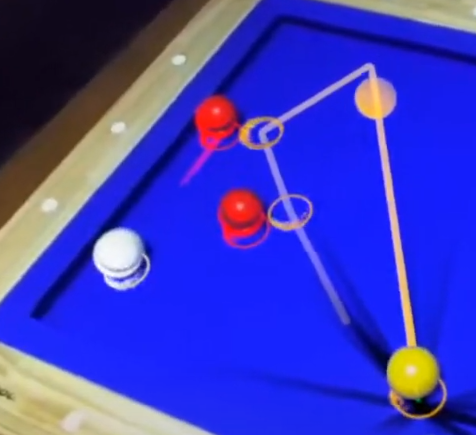
\includegraphics[width=5cm]{img/abstract-final.png}
\end{figure}

\begin{abstract}
    당구는 재미있는 실내 스포츠이지만, 지금처럼 오락거리가 많은 시대에 초심자가 발을 붙이기에는 다소 진입장벽이 높다. AR 당구는 입문자들이 당구의 높은 진입장벽을 손쉽게 극복하는 데 도움을 줄 수 있도록 기획되었다. 몰입도 높은 VR HMD \footnotemark 상에서 당구공이 득점 가능한 최적의 경로 및 사용자가 취한 큐의 각도에 대한 피드백을 시각화하고, 여러 시청각 효과를 통한 오락 요소를 도입하여 입문자의 흥미 유발과 당구에 대한 감각 습득을 돕는다.
    \footnotetext{Head Mounted Display의 약자; VR 헤드셋과 같이 머리에 장착하여 사용자의 시야 전체를 채우는 형태의 장착형 디스플레이 기기를 일컬음}

    AR 당구의 구현은 (1) 영상 처리를 통한 당구대, 당구공, 큐의 3D Pose 획득 (2) 득점 경로를 계산하기 위한 물리 시뮬레이션 구현 (3) 오브젝트의 3D 포즈 및 계산된 득점 경로 등에 대한 시각화의 세 요소를 통해 이루어진다.

    (Abstract 내 최종 구현 내용은 추후 기술)
\end{abstract}

\newpage

% \twocolumn[]
\section{영상 처리}
\subsection{개요}
가상 현실\textss{Vritual Reality} 기술은 말 그대로 가상으로 세계를 만들고, 헤드 트래킹 기술을 통해 가상 세계의 카메라 위치를 사용자 눈의 위치와 동기화하여 사실적인 시청각 경험을 부여하는 기술이다.

\begin{figure}[ht]
    \begin{center}
        \begin{subfigure}{0.4\textwidth}
            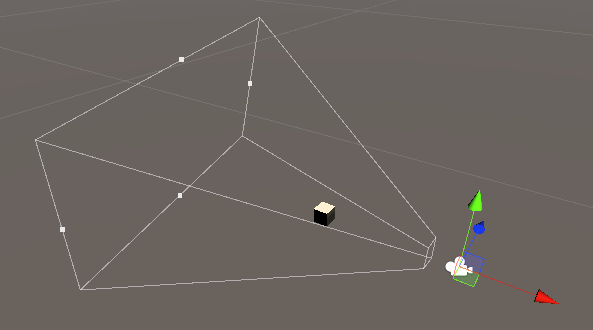
\includegraphics[width=\textwidth]{img/vr-example-camera.png}
            \caption{}
        \end{subfigure}
        \begin{subfigure}{0.4\textwidth}
            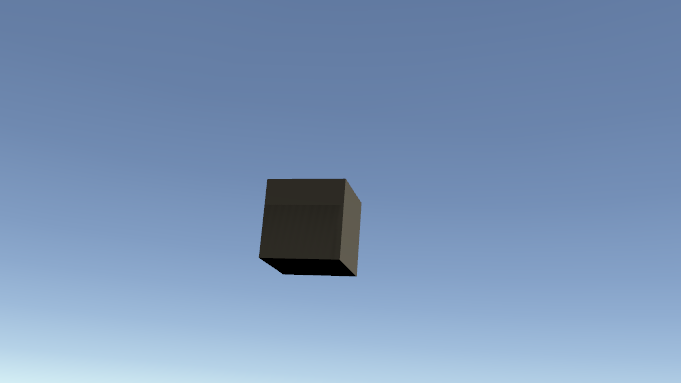
\includegraphics[width=\textwidth]{img/vr-example-view.png}
            \caption{}
        \end{subfigure}
        \caption{가상 세계의 카메라가 사용자의 머리 위치에 따라 동기되어 현실적인 느낌을 준다}
    \end{center}
\end{figure}

가상 현실 어플리케이션은 기존의 전통적인 3D 게임에서 카메라의 제어만을 사용자가 장착한 HMD의 헤드 트래킹 신호에 위임한 것으로, 가상 현실 세계를 만드는 것은 3D 게임을 만드는 것과 다르지 않다.

본 과제에서 구현한 증강 현실\textss{Augmented Reality} 어플리케이션 또한 이 개념에서 크게 벗어나지 않는다. 여전히 가상 세계의 좌표와 카메라 위치 동기화 및 오브젝트 배치가 필요하며, 이들 오브젝트를 현실 세계의 영상 위에 덧그린다는 것이 가상 현실과의 유일한 차이점이다.

그러나 증강 현실 어플리케이션이 설득력을 얻기 위해서는 덧그린 가상 현실 오브젝트의 위치와 크기, 모양 등이 영상의 물체와 보기 좋게 어우러져야 하므로, 영상 처리를 통해 현실 세계의 오브젝트가 가상 세계의 어느 트랜스폼으로 매핑되는지 파악하는 것이 중요하다.

한 번 현실 세계 오브젝트의 가상 세계 좌표를 획득하고 나면, 이후에는 해당 좌표에 가상 오브젝트를 생성하는 것만으로도 증강 현실 영상에 그럴싸한 효과를 그려낼 수 있게 된다. 단, 해당 오브젝트가 지속적으로 움직이고 있는 상태라면 지속적으로 영상 처리를 수행해 해당 오브젝트의 가상 현실 좌표를 업데이트 해주어야 할 것이다.

AR 당구의 영상 처리 또한 이러한 맥락에서 동작한다. 당구대와 당구공의 가상 세계 좌표를 획득하면 게임 엔진은 이 정보를 바탕으로 당구공이나 당구대에 대한 오버레이를 그리거나, 당구공의 최적 타격 경로에 대한 시뮬레이션 등을 수행하고 이 결과를 시각화하는 등 여러 방향으로 활용할 수 있다.

영상 처리 절에서는 일차적으로 영상 처리를 통해 당구대와 당구공 등 각 물체의 카메라에 대한 3D 포즈를 계산하고, 이를 가상 세계의 좌표로 변환하는 과정을 다룬다.

\subsection{당구대 인식}
\subsubsection{필터링}
\label{section;imgproc;table}
\begin{figure}[ht]
    \centering
    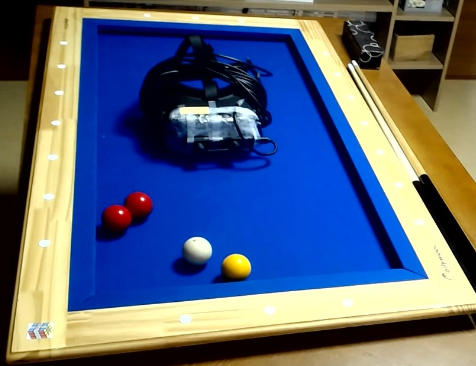
\includegraphics[width=8cm, height=8cm, keepaspectratio]{img/billiards-table.png}
    \caption[Caption for LOF]{당구대 세트, VR HMD 및 HMD에 장착된 스테레오 카메라\footnotemark}
    \label{fig;pool-table}
\end{figure}
\footnotetext{휴대성, 작업의 용이성, 경제성 등을 고려하여 작은 크기의 미니 당구 세트를 활용하였다.}

\cref{fig;pool-table}에서 당구대 펠트의 진한 파란색이 매우 뚜렷하다. 색감이 이렇게 강한 물체는 HSV 색공간으로 표현했을 때  hue 영역이 안정적으로 고정되고, saturation이 강해 다른 영역과 쉽게 구별할 수 있다(\cref{fig;pool-table-hs}).

\begin{figure}[ht]
    \centering
    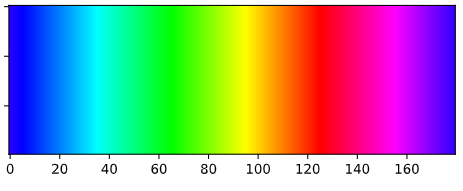
\includegraphics[width=8cm]{img/hsv-spectrum.png}
    \caption{OpenCV의 HSV 스펙트럼 (8-bit)}
    \label{fig;hsv-spectrum}
\end{figure}

\begin{figure}[ht]
    \centering
    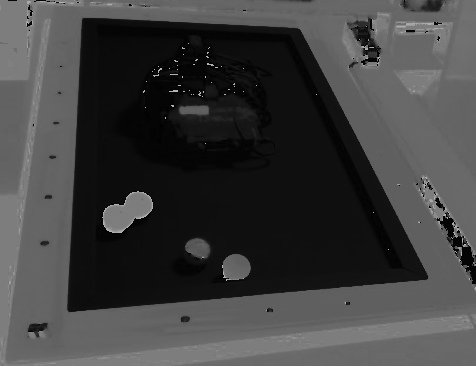
\includegraphics[width=5cm, height=5cm, keepaspectratio]{img/billiards-table-h-shift.png}
    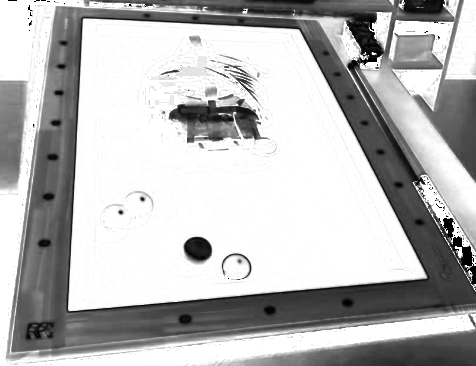
\includegraphics[width=5cm, height=5cm, keepaspectratio]{img/billiards-table-s.png}
    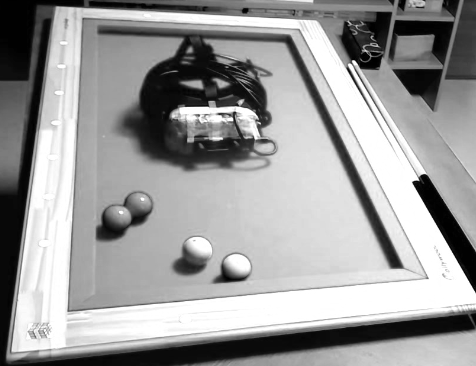
\includegraphics[width=5cm, height=5cm, keepaspectratio]{img/billiards-table-v.png}
    \caption[Caption for LOF]{\cref{fig;pool-table}의 HSV 색공간 변환 이미지. 순서대로 H\footnotemark, S, V. 검은색은 0, 흰색은 255 범위}
    \label{fig;pool-table-hs}
\end{figure}

\cref{fig;pool-table-hs}의 hue 영역 이미지의 각 픽셀 값은 \cref{fig;hsv-spectrum}의 스펙트럼에 대응한다. 따라서 hue 값이 약 0$\sim$25 사이에 분포하는 픽셀을 필터링하면 당구대 영역을 식별할 수 있다. 그러나 saturation이 현저히 낮아 색상을 구별할 수 없는 흰색과 검은색은 hue 값이 단순히 0에 매핑되므로, hue 값만을 사용해 필터링할 경우 잘못된 결과를 얻을 수 있다. 따라서 saturation 값 또한 일정 이상의 값(170$\sim$255)을 갖는 픽셀을 선택한다.

Value(밝기)는 당구대 영역을 식별하는 데 큰 도움을 주진 않으므로, 모든 범위를 선택한다.

\begin{figure}[ht]
    \centering
    \begin{subfigure}{0.4\textwidth}
        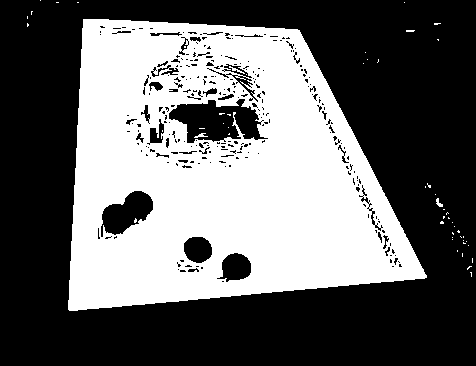
\includegraphics[width=\textwidth]{img/billiards-table-filter.png}
        \caption{필터링된 이진 이미지}
        \label{fig;pool-table-edge-a}
    \end{subfigure}
    \begin{subfigure}{0.4\textwidth}
        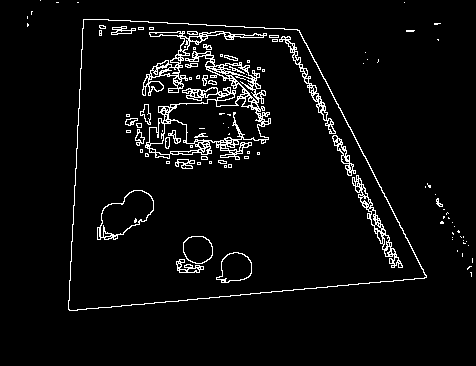
\includegraphics[width=\textwidth]{img/billiards-table-edge.png}
        \caption{검출된 경계선}
        \label{fig;pool-table-edge-b}
    \end{subfigure}
    \caption{}
    \label{fig;pool-table-edge}
\end{figure}

\footnotetext{이 때, Hue 채널은 파란색이 0도와 180도 양단에 걸쳐 있어 5\si{\degree} 우측으로 전이\textss{shift}하였다}

\cref{fig;pool-table-edge}의 왼쪽 이미지가 위에서 말한 필터링을 적용한 결과이다. \footnotemark 여러 가지 물체가 당구대 위에 올려져 있고, 당구대의 쿠션 밑에 생긴 음영 등으로 인해 당구대의 펠트 전체가 깔끔하게 덮이지는 않았지만, 당구대 영역을 식별하는 것은 가능하다.
\footnotetext{OpenCV의 inRange 함수를 사용한다. 함수 inRange는 이미지의 각 채널(여기서는 H, S, V)에 대해 필터링할 값의 범위를 지정하고, 각 픽셀이 해당 범위 내에 속하는지 여부를 검사해 부울\textss{bool} 값으로 반환한다.}

\subsubsection{정점 검출}
그러나 이 시점에서 \cref{fig;pool-table-edge-a}의 이진 이미지는 단순힌 부울 값 배열로, 이미지만 놓고 봤을 때 프로그램은 당구대 영역의 위치는 물론, 존재 여부조차 알 수 없다. 따라서 이미지에서 당구대를 이루는 영역이 어디인지를 찾고 처리하기 쉬운 형태로 표현하기 위해 이미지 상에 존재하는 모든 도형을 찾고, 당구대의 조건에 부합하는 도형을 선택하기로 한다. 여기서는 픽셀 면적이 일정 이상이고, 꼭지점의 개수가 정확히 4개인 도형을 찾는다.

먼저 이미지의 경계선 정보가 필요하다. 이진 이미지에 침식 연산\footnotemark을 적용한 후, 원본 이미지에서 침식된 이미지를 빼는 것으로 각 덩어리\textss{chunk}의 경계선만을 남길 수 있다. \cref{fig;pool-table-edge-b}가 이에 해당한다.
\footnotetext{이진 이미지에서, 값이 1인 각각의 픽셀을 인접한 픽셀들과 평가하여, 인접한 픽셀 모두 1이면 1로, 하나라도 0이면 0으로 바꾸는 연산. 노이즈 제거 등에 활용한다}

경계선 이미지에 OpenCV의 findContours 함수를 적용한다.\cite{findContours} findContours는 이진 이미지에 존재하는 모든 닫힌 도형 목록을 찾아 반환하는 함수로, 하나의 도형(등고선\textss{contour}으로 표현)은 그 도형을 이루는 정점의 좌표 목록으로 구성된다.

이 때 함수가 가장 바깥쪽의 도형만 탐색하게끔 인자를 지정한다. \cref{fig;pool-table-edge-b}의 당구공, HMD, 쿠션의 음영 등으로 인해 생긴 도형들은 모두 가장 바깥쪽의 당구대 영역 내부에 존재하므로 도형 탐색 과정에서 고려하지 않는다. 이로써 당구대 내부에 생기는 어느 정도의 잡음은 무시할 수 있게 된다.

그러나 이렇게 획득한 등고선의 정점 목록을 그대로 평가하기에는 다소 어려움이 있는데, OpenCV의 findContours 함수는 두 점 사이의 직선성을 매우 엄격하게 평가하기 때문이다. 즉, \cref{fig;pool-table-edge-b}의 당구대 경계선은 육안으로는 4개의 꼭지점을 잇는 사각형으로 보이지만, 픽셀 단위로 처리될 땐 곧은 직선이 아닌 여러 정점을 갖는 파선으로 평가될 수 있는 것이다.

\begin{figure}[ht]
    \centering
    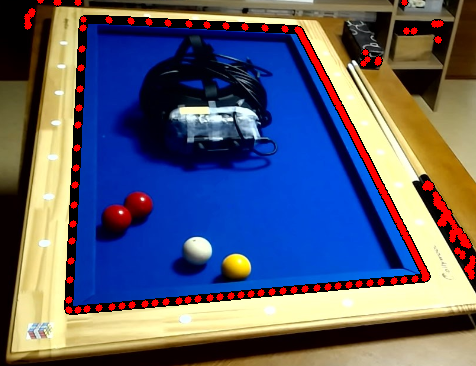
\includegraphics[width=8cm]{img/billiards-table-contours-dot-view.png}
    \caption{각각의 붉은 점은 정점을, 검은 선은 정점을 잇는 간선을 나타낸다}
    \label{fig;table-contour-dot-view}
\end{figure}

\cref{fig;table-contour-dot-view}는 이를 잘 나타낸다. 당구대 영역을 구성하는 도형의 한 변은 직선이 아닌 무수한 정점을 지나는 파선으로 평가된다. 우리는 꼭지점의 개수(4개)를 통해 당구대 영역을 찾고자 하므로, 융통성 없게 평가된 등고선의 정점 목록을 직선이 되도록 어느 정도 근사해주어야 한다.

여기에는 OpenCV의 approxPolyDP\footnotemark 함수를 사용한다. 이 때 approxPolyDP 함수에서 근사의 민감도를 나타내는 인자인 $\epsilon$은 픽셀 단위인데, 많은 경우 당구대의 직선은 10픽셀 이상 벗어나지 않는 깔끔한 형태를 보이므로 epsilon은 10으로 설정한다. 그 결과 \cref{fig;table-contour-dot-view-approx}과 같이 당구대 영역의 정점 개수가 4개로 정리되고, 4개의 정점을 이은 도형이 나타내는 영역 또한 당구대 영역에 잘 맞음을 확인할 수 있다.
\footnotetext{\textit{Ramer–Douglas–Peucker algorithm}의 구현체. 시점과 종점을 잇는 간선이 잇는 두 정점 사이의 정점 목록 중 가장 거리가 먼 정점이 임계점 $\epsilon$보다 멀리 있으면 해당 정점을 새로운 종점으로 선택하고, 가까이 있으면 해당 정점을 제거하고 기존의 종점을 시점으로 선택해 새 간선으로 위의 과정을 재귀적으로 반복, 근사를 수행하는 알고리즘이다.}

\begin{figure}[ht]
    \centering
    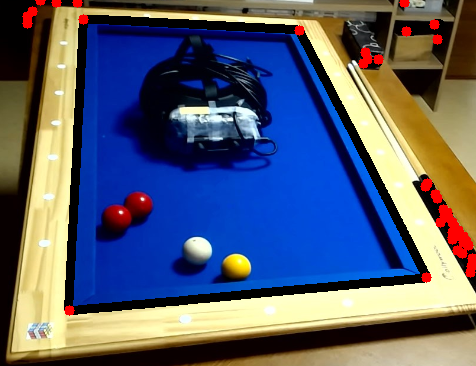
\includegraphics[width=8cm]{img/billiards-table-contours-dot-view-approx.png}
    \caption{$\epsilon=10$으로 approxPolyDP 함수를 적용한 경우의 시각화}
    \label{fig;table-contour-dot-view-approx}
\end{figure}

그러나 위와 같은 방법으로 당구대 영역을 계산하는 경우, 당구대 영역을 침범하는 작은 잡음에도 매우 취약해지는 문제가 발생한다. AR HMD를 착용하고 당구를 즐기는 사용자의 시점에서 큐가 당구대 영역 안으로 들어가거나 입체인 공이 당구대의 경계를 가리는 등 당구대의 경계선이 왜곡되는 일은 매우 빈번하게 발생한다(당구대의 일부만이 시야에 들어오는 경우는 뒤에서 다룬다).

\begin{figure}[ht]
    \centering
    \begin{subfigure}{8cm}
        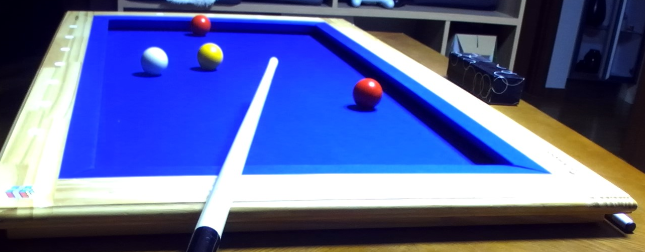
\includegraphics[width=\textwidth]{img/billiards-table-low-angle.png}
        \caption{}
        \label{fig;table-lowangle-src}
    \end{subfigure}
    \centering
    \begin{subfigure}{8cm}
        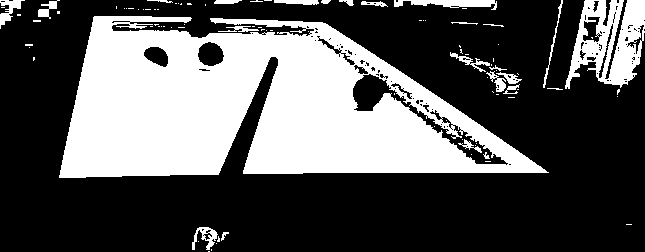
\includegraphics[width=\textwidth]{img/billiards-table-low-angle-flt.png}
        \caption{}
        \label{fig;table-lowangle-flt}
    \end{subfigure}
    \centering
    \begin{subfigure}{8cm}
        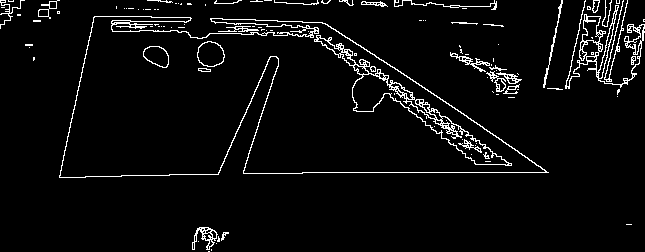
\includegraphics[width=\textwidth]{img/billiards-table-low-angle-edge.png}
        \caption{}
        \label{fig;table-lowangle-edge}
    \end{subfigure}
    \centering
    \begin{subfigure}{8cm}
        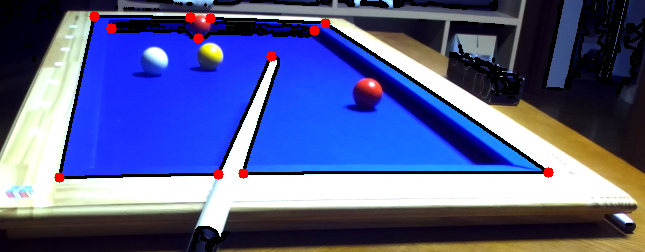
\includegraphics[width=\textwidth]{img/billiards-table-low-angle-approx.png}
        \caption{}
        \label{fig;table-lowangle-aprx}
    \end{subfigure}
    \caption{}
    \label{fig;table-lowangle}
\end{figure}

\cref{fig;table-lowangle}은 이렇게 당구대의 경계가 침범당할 때의 처리 과정을 보여주는 이미지로, \cref{fig;table-lowangle-edge}에서 당구대의 침범 당한 경계선을 따라 \cref{fig;table-lowangle-aprx}의 등고선이 형성되었음을 볼 수 있다. 특히 \cref{fig;table-lowangle-aprx}의 위쪽, 빨간 공에 의해 침범당한 부분은 공이 내부의 쿠션 음영으로 인한 잡음와 당구대의 외부 경계를 잇는 가교 역할을 해, 더 나쁜 결과를 반환한다.

단순히 정점의 개수가 4개이며, 넓이가 일정 이상이면서 가장 큰 도형을 당구대의 영역으로 판단하는데, 당구대 영역의 도형이 \cref{fig;table-lowangle-aprx}와 같이 계산되면 이를 당구대 영역으로 인식하지 못하게 된다.

그러나 \cref{fig;table-lowangle-aprx}에서 검출된 정점 중 가장 바깥쪽의 정점 4개를 이어보면 여전히 내부의 다른 모든 정점을 포함하는 볼록 다각형\textss{convex hull}을 획득할 수 있다. 다행히도 OpenCV 라이브러리에는 정점 목록으로부터 볼록 다각형을 계산해내는 함수성 또한 포함되어 있어, 이를 적용한 결과는 \cref{fig;table-lowangle-convexhull}과 같다.

이 때 조금이라도 돌출된 부분이 있다면 \cref{fig;table-lowangle-convexhull-src}와 같이 돌출된 부분을 새로운 정점으로 계산하게 되므로, 정점의 개수를 다시 4개로 근사하기 위해 예의 approxPolyDP 함수를 다시 적용, \cref{fig;table-lowangle-convexhull-aprx}를 얻는다.

\begin{figure}[ht]
    \centering
    \begin{subfigure}{8cm}
        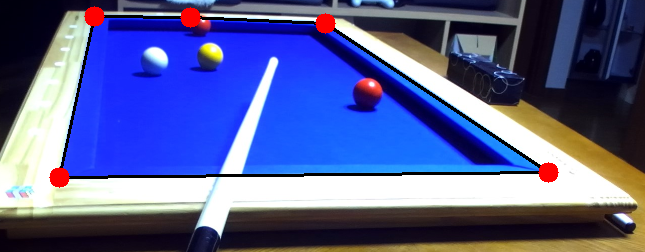
\includegraphics[width=\textwidth]{img/billiards-table-low-angle-convex.png}
        \caption{}
        \label{fig;table-lowangle-convexhull-src}
    \end{subfigure}
    \begin{subfigure}{8cm}
        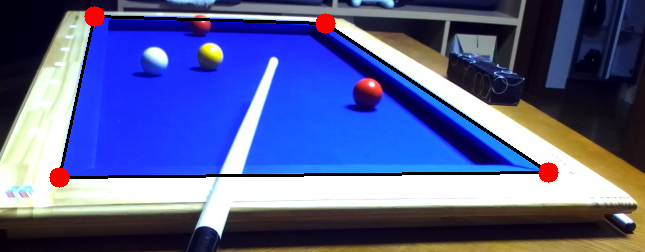
\includegraphics[width=\textwidth]{img/billiards-table-low-angle-convex-aprx.png}
        \caption{$\epsilon=10$으로 approxPolyDP 함수 재적용}
        \label{fig;table-lowangle-convexhull-aprx}
    \end{subfigure}
    \caption{convex hull 적용}
    \label{fig;table-lowangle-convexhull}
\end{figure}

이렇게 얻어진 당구대 영역의 사각형은(바로 앞에 파랗고 커다란 직사각형 물체를 갖다 놓지 않는 한) 대체로 찾아낸 사각형 중 가장 큰 크기를 갖게 되므로, 사각형을 이루는 네 개의 정점이 당구대의 네 귀퉁이에 해당한다고 안전하게 가정할 수 있다.

\subsubsection{포즈 추정\textss{pose estimation}}
당구대의 펠트에 해당하는, 바깥 쿠션 영역의 치수는 $0.96 \times 0.52[m]$이다. 만약 카메라의 위치에 같은 크기의 직사각형 판이 있다고 가정하면, 이를 적절하게 회전시키고 이동시켜 화면 상의 당구대 펠트 영역을 정확하게 덮을 수 있을 것이다. 이 때의 직사각형 판을 모델이라 하면, 화면 상의 펠트 영역을 덮기 위해 모델에 적용할 회전과 이동이 당구대의 포즈\textss{pose}가 된다.

당구대의 치수를 알고 있기 때문에 모델 공간(원점)에 존재하는 당구대의 4개 정점을 설정할 수 있다. 당구대의 모델은 ZX 평면에 가로로 배치하기로 한다. 즉, 네 개 정점의 좌표는 원점 $(x,y,z)=(0,0,0)$에 대해 $$\abs{x}=0.48,\;\;\abs{y}=0,\;\;\abs{z}=0.26 _{[m]}$$가 된다.

OpenCV의 좌표 공간은 보는 방향의 오른쪽을 X, 아래쪽을 Y축, 정면을 Z축으로 하는 오른손 좌표계를 사용한다. 따라서 ZX 평면에 놓인 모델 공간의 당구대는 시선에 수평이며, \cref{fig;table-3d-model}에서와 같이 각 정점은 왼쪽 앞부터 반시계 방향으로 배치된다.

\begin{figure}[ht]
    \centering
    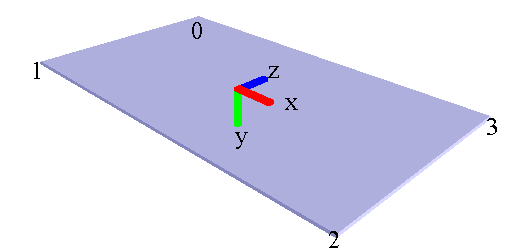
\includegraphics[width=8cm]{img/table-3d.pdf}
    \caption{모델 공간의 당구대 정점 배치}
    \label{fig;table-3d-model}
\end{figure}

당구대의 모델을 설정하였으므로 이 모델을 임의로 이동하고 회전시킨 뒤, 카메라 내부 파라미터 값을\textss{cam\-era intrinsic parametter} 바탕으로 화면에 투영하면 투영된 각 점과 이미지에서 검출된 당구대의 네 정점 사이의 오차를 구할 수 있다. 이 과정을 점진적으로 반복하여 오차를 줄여나가, 최종적으로 정확한 당구대의 포즈를 구하는 것이 포즈 추정 알고리즘의 골자이다.

\begin{figure}[ht]
    \begin{center}
        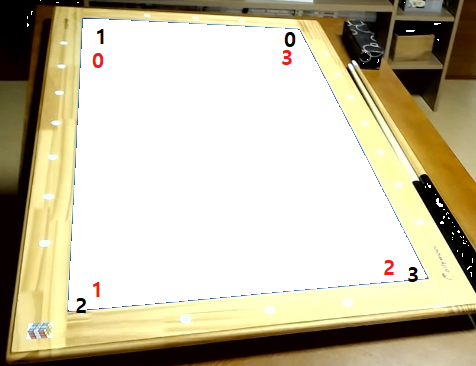
\includegraphics[width=8cm, height=5cm, keepaspectratio]{img/billiards-table-indexes.png}
    \end{center}
    \caption{바깥쪽 숫자는 레퍼런스, 안쪽 숫자는 검출된 정점 순서}
    \label{fig;pool-table-invalid-index}
\end{figure}

그러나 본격적으로 포즈 추정 알고리즘을 적용하기 전 해결해주어야 하는 문제가 있다. \cref{fig;pool-table-invalid-index}에서와 같이, 실제 검출된 인덱스의 순서가(단, 인덱스의 회전은 convexHull 함수에 의해 항상 반시계 방향으로 고정된다) 홀수 개수;1개 또는 3개 만큼 밀릴 수 있다. 

당구대는 직사각형 모양이므로, 긴 변과 짧은 변은 엄격하게 구별되어야 한다. 그러나 \cref{fig;pool-table-invalid-index}에서와 같이 인덱스의 순서가 홀수 개수로 틀어지게 되면(2개 밀린 경우, 단순히 결과물에 180\si{\degree} 회전을 가하면 된다) 포즈 추정 알고리즘은 긴 변과 짧은 변을 반대로 인식하여 잘못된 결과를 반환하게 된다.

따라서 이미지에 포즈 추정 알고리즘을 적용하기 전, 먼저 인덱스의 정합\textss{alignment}을 검증해야 한다. 그러나 단순히 2D 이미지 상에서의 유클리드 거리로 인덱스를 정렬하려 하면, 당구대의 긴 변과 짧은 변은 시점에 따라 잘못된 결과를 반환한다(예를 들어, \cref{fig;table-lowangle-convexhull-aprx}의 아래쪽 짧은 변이 왼쪽의 긴 변보다 더 길게 측정된다). 따라서 정확한 비교를 위해 스테레오 카메라\footnote{ZED Mini를 사용}로부터 획득한 깊이 이미지를 활용한다.

\begin{figure}[ht]
    \centering
    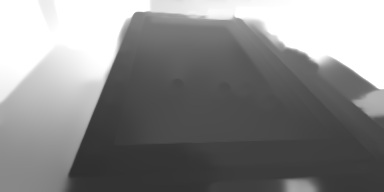
\includegraphics[width=8cm]{img/table-depth.png}
    \caption{ZED Mini에서 생성된 깊이 이미지 (다른 앵글)}
    \label{fig;table-depth-image}
\end{figure}

\cref{fig;table-depth-image}에서 각 픽셀 좌표에 해당하는 깊이 값을 얻을 수 있다. 깊이 값 z를 알면, 카메라의 내부 파라미터를 이용해 픽셀 좌표 u, v로부터 3D 공간의 좌표 x, y를 계산해낼 수 있다. 이 때의 식은 \cref{eq;xyz-from-uvz}과 같다.

\begin{align} 
    \begin{split}
        x &= z\cdot\frac{u-c_x}{f_x} \\
        y &= z\cdot\frac{v-c_y}{f_y} 
    \end{split}
    \label{eq;xyz-from-uvz}
\end{align}

이를 통해 이미지에서 검출된 당구대 각 정점의 3D 좌표를 계산할 수 있으며, 이를 바탕으로 짧은 변이 먼저 나타나게끔 검출된 정점의 인덱스를 재정렬하면 포즈 추정 알고리즘을 적용할 준비가 완료된다.

OpenCV 라이브러리는 직접 반복적인 탐색을 구현하는 것보다 더 효과적이고 정확하게 포즈를 찾아내는 알고리즘 구현체를 다수 제공한다. 이러한 알고리즘들은 solvePnP라는 함수에 인자를 제공하는 형태로 활용할 수 있다.\footnote{여기서는 iterative 방법을 지정한다. Levenberg-Marquardt optimization 알고리즘을 활용해 최적해를 찾는 구현체}

당구대 모델의 네 정점의 좌표 목록과 화면 상의 당구대 정점 목록, 카메라 내부 파라미터를 인자로 solve\-PnP 함수를 호출하면 카메라에 대한 당구대의 포즈; 위치와 회전 벡터를 획득할 수 있다.

일종의 안전 장치로써 OpenCV의 projectPoints 함수를 활용, 모델을 추정 포즈로 다시 화면에 투영하여 각 정점의 오차의 최대값을 구한다. 오차가 일정 이하일 때에만 이를 당구대의 포즈로 결정한다.

최종적으로 획득한 포즈는 카메라에 대한 상대 포즈이며, 여기서 카메라는 HMD를 쓴 사용자의 머리 위치를 일컫는다. 카메라 또한 가상 세계의 월드 원점에 대한 트랜스폼을 갖고 있으므로, 앞서 계산한 당구대의 포즈에 카메라 트랜스폼을 적용하면 당구대의 월드 좌표와 회전을 획득할 수 있다.

\subsubsection{당구대의 일부만 시야에 들어온 경우}

당구대는 보통 움직이지 않으므로, 한 번 인식한 당구대의 월드 위치는 불변이어야 한다. 이상적으론 당구대를 인식할 수 없는 상황에서도 장치의 헤드 트래킹 기능을 활용해 카메라에 대한 당구대의 상대 위치는 지속적으로 파악할 수 있어야 한다.

그러나 기술적인 문제\footnotemark로 인해 장치의 헤드 트래킹 기능이 보고한 카메라의 월드 위치를 완전히 신뢰하기는 어려우므로, 당구대의 포즈를 지속적으로 인식하여 헤드 트래커의 오차를 보정해주어야 한다.
    \footnotetext{과제는 Oculus Rift의 첫 상업용 버전을 활용한다. 이 버전의 Rift는 두 개의 고정 센서 및 HMD에 내장된 IMU를 활용해 위치를 추정하는데, 항상 위치의 절대값을 보고하므로 오차 누적(drift) 문제에서는 자유롭다. 그러나 절대값 자체에 경미한 오류가 있어, 사용자의 위치가 바뀌면 당구대의 위치가 약간 어긋나게 보인다. 

    Oculus Rift를 AR 기기로 활용하기 위해 장착한 ZED Mini 또한 IMU 및 공간 매핑\textsubscript{spatial mapping} 기능을 통한 헤드 트래킹 기능을 제공한다. 그러나 공간 매핑 기능의 IMU 오차 누적 보정이 너무 불연속적이고 품질이 나빠 비활성화하였기 때문에 결국 오차 누적 문제를 안고 가게 되었다.}

보통 당구를 즐기는 사용자 시점에서, 당구대 전체가 시야에 들어오는 경우는 비율로 따지면 적은 편이다. 사용자는 대부분의 시간 동안 \cref{fig;table-partial}과 같이 당구대의 일부만을 볼 수 있고, 이 경우 PNP 알고리즘을 적용할 네 개의 정점을 온전하게 획득하는 것은 다소 어렵다. 

하지만 OpenCV에서 제공하는 세련된 방법을 사용하지 못한다는 제약이 생길 뿐이며, 당구대의 모델에 특정한 포즈를 취해 화면상의 검출된 점과 정합시킬 수 있다는 사실에는 변함이 없다. 따라서 임의의 포즈를 지정, 투영하며 반복적으로 오차를 줄여나가는 포즈 추정 알고리즘을 직접 구현하기로 한다.

\begin{figure}
    \centering 
    \begin{subfigure}{3.5cm}
        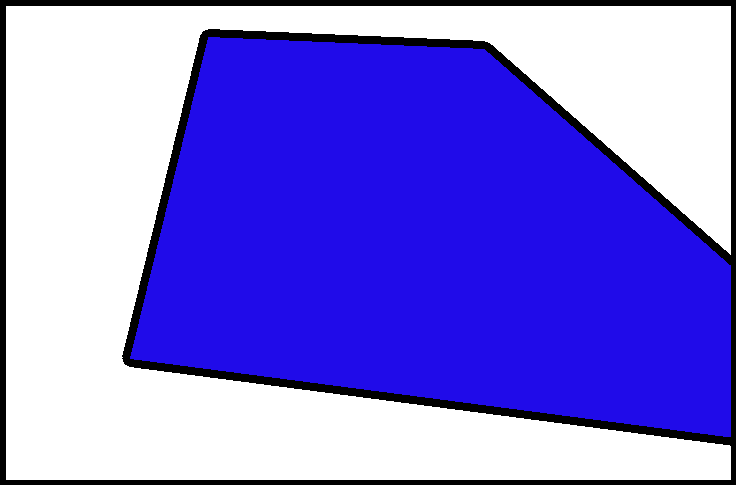
\includegraphics[width=\textwidth]{img/table-partial-view-filter-0.png}
        \caption{}
        \label{fig;table-partial-0}
    \end{subfigure}
    \begin{subfigure}{3.5cm}
        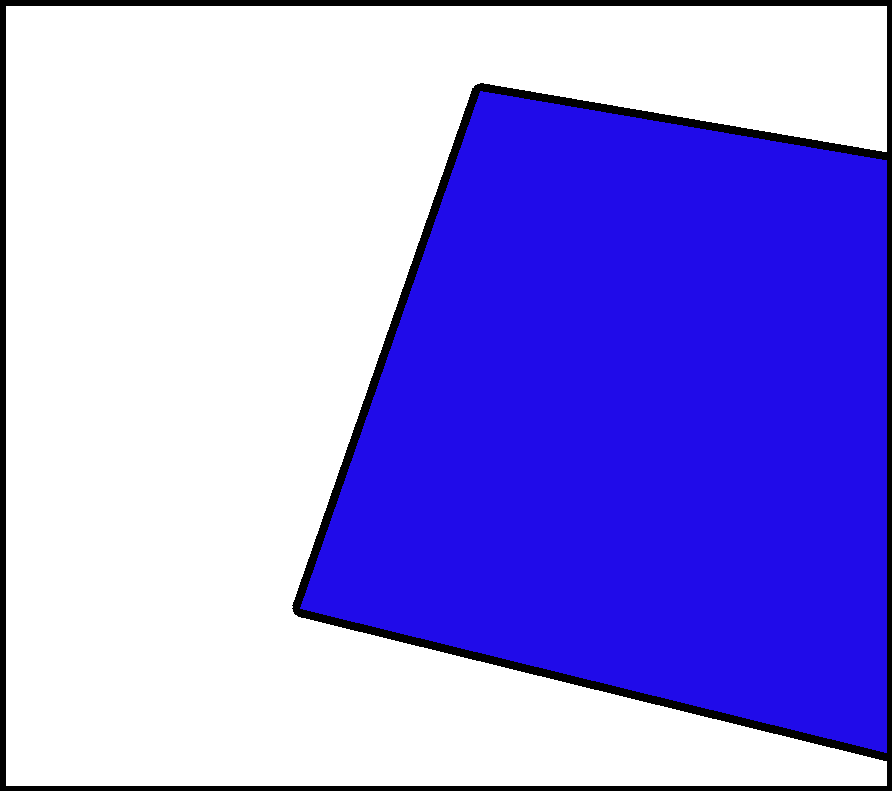
\includegraphics[width=\textwidth]{img/table-partial-view-filter-1.png}
        \caption{}
        \label{fig;table-partial-1}
    \end{subfigure}
    \begin{subfigure}{3.5cm}
        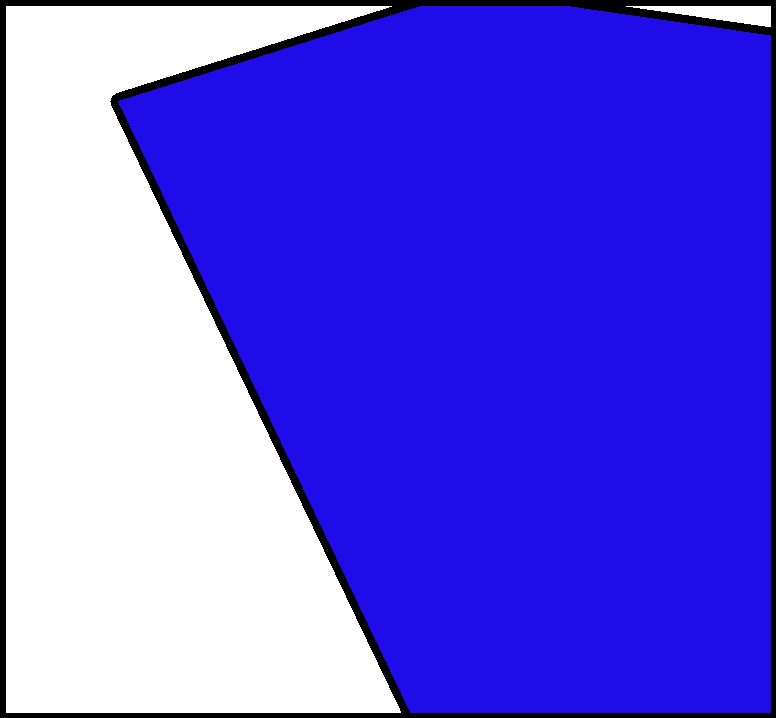
\includegraphics[width=\textwidth]{img/table-partial-view-filter-3.png}
        \caption{}
        \label{fig;table-partial-3}
    \end{subfigure}
    \begin{subfigure}{3.5cm}
        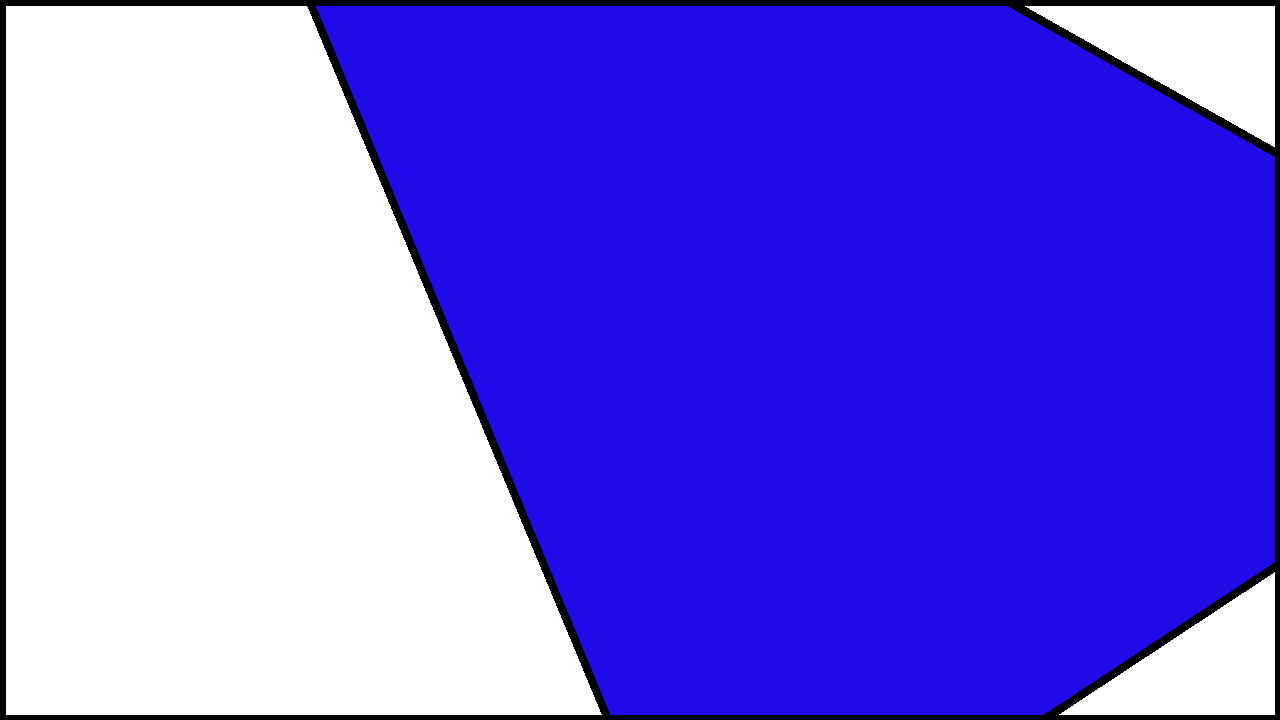
\includegraphics[width=\textwidth]{img/table-partial-view-filter-4.png}
        \caption{}
        \label{fig;table-partial-4}
    \end{subfigure}
    \begin{subfigure}{3.5cm}
        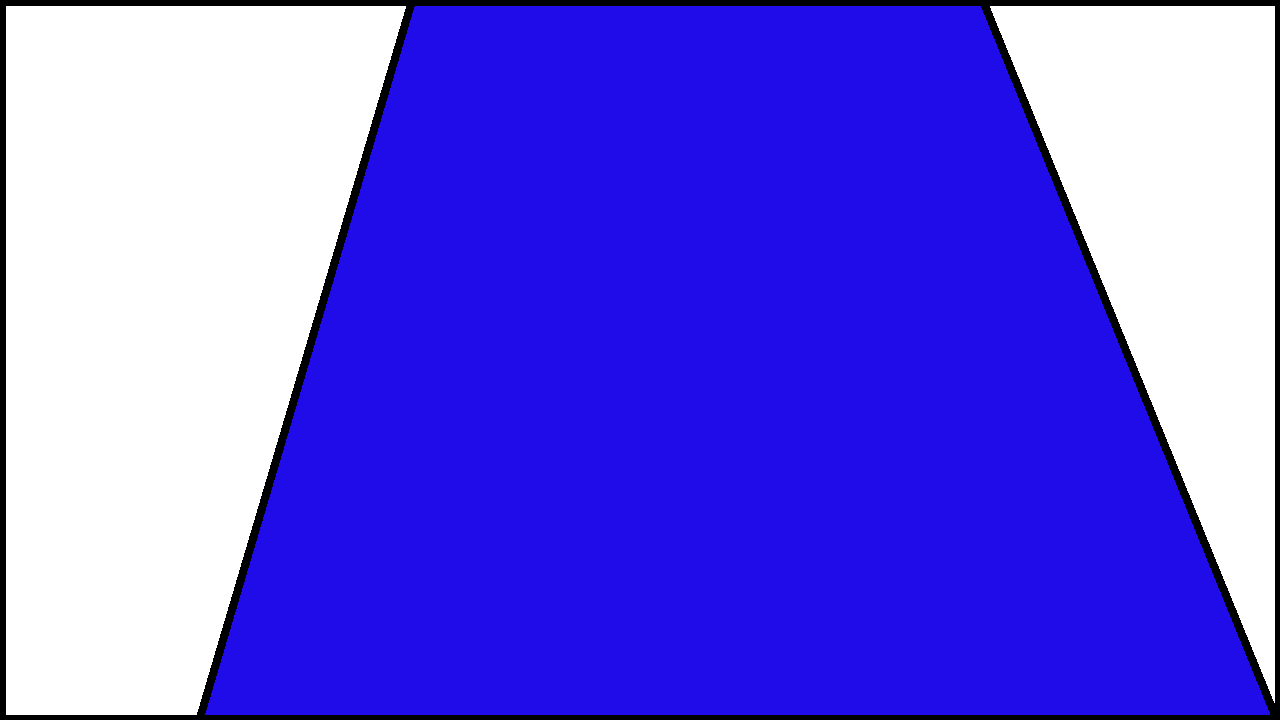
\includegraphics[width=\textwidth]{img/table-partial-view-filter-5.png}
        \caption{}
        \label{fig;table-partial-5-disable}
    \end{subfigure}
    \begin{subfigure}{3.5cm}
        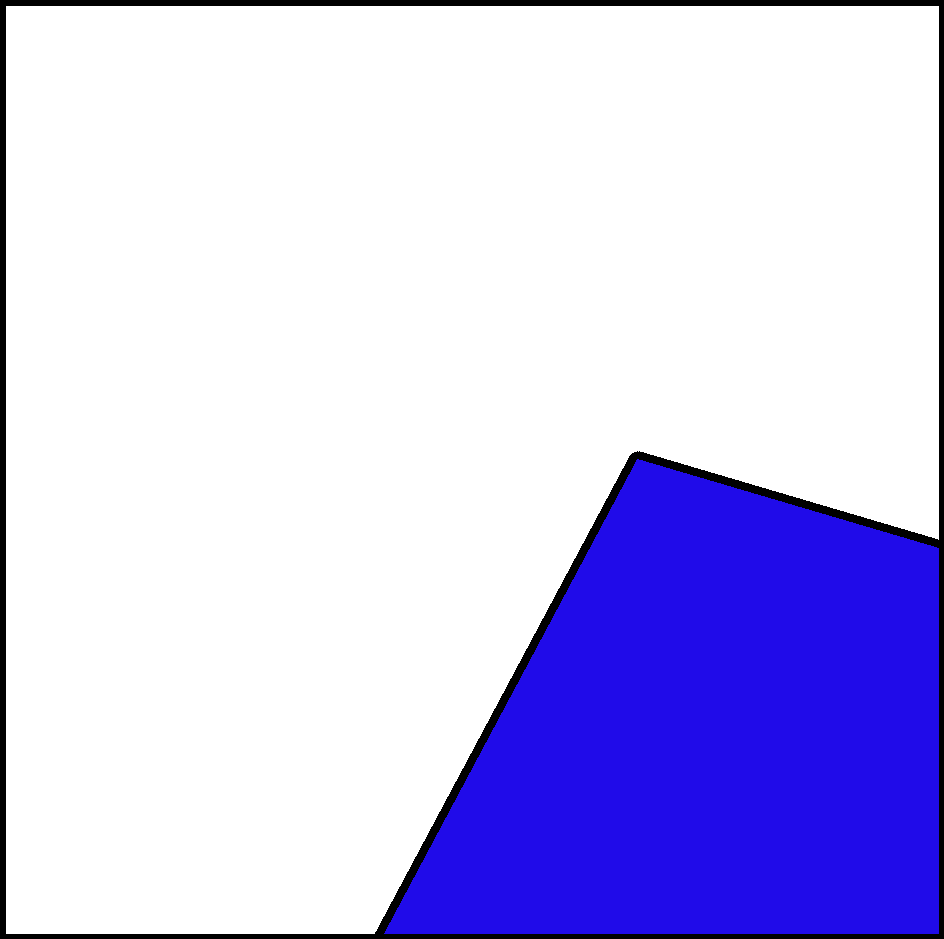
\includegraphics[width=\textwidth]{img/table-partial-view-filter-2.png}
        \caption{}
        \label{fig;table-partial-2-disable}
    \end{subfigure}
    \caption{당구대의 일부만 검출}
    \label{fig;table-partial}
\end{figure}

\cref{fig;table-partial}은 당구대의 일부만이 시야에 들어오는 경우를 나타낸다. 단, \cref{fig;table-partial-5-disable}과 \cref{fig;table-partial-2-disable}의 경우 해당 도형에 정합시킬 수 있는 당구대의 포즈가 무수히 존재한다. 

유한한 개수의 포즈를 획득할 수 있는 도형을 찾기 위해 간단한 조건을 설정한다. 이미지의 경계선에 접해있는 점의 가중치를 1, 접해있지 않은(당구대의 꼭지점에 해당) 점의 가중치를 2로 두어, 검출된 모든 정점의 가중치의 합이 6 이상인 도형에 대해서만 탐색을 수행한다. 

탐색은 당구대 모델에 임의의 포즈를 적용하고 화면에 투영한 뒤, 각 정점의 위치를 비교하는 방식으로 이루어진다. 

단, 화면에 투영하기 전 추가적인 처리가 필요하다. 당구대 모델에 추정 포즈를 적용한 경우 공간 상에서 당구대는 \cref{fig;invalid-sight-projection}와 같은 모습으로 배치된다. 

\begin{figure}[ht]
    \centering
    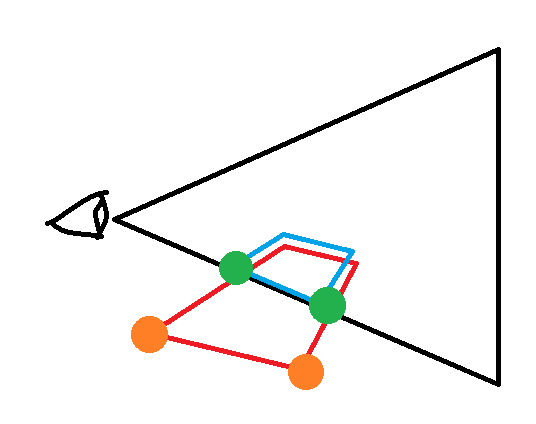
\includegraphics[width=7cm]{img/sight-invalid-culling.png}
    \caption{삼각형은 카메라의 시야 영역}
    \label{fig;invalid-sight-projection}
\end{figure}

\begin{comment}

당구대의 일부만이 시야 내에 있어 컨투어의 정점 개수가 5개 이상 검출되는 경우에는 PNP 알고리즘을 적용할 정확한 정점의 위치를 파악하기 어렵다. 하지만, 적어도 두 개 이상의 코너가 시야 내에 잡혔다면 당구대의 포즈를 추정하는 것이 가능하다.

\begin{figure}[h]
    \centering
    \begin{subfigure}{0.4\textwidth}
        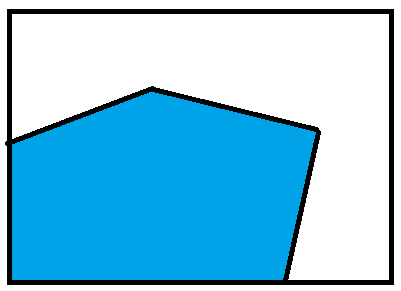
\includegraphics[width=\textwidth]{img/partial-table-valid-case.png}
        \caption{위치를 추정할 수 있음}
    \end{subfigure}
    \centering
    \begin{subfigure}{0.4\textwidth}
        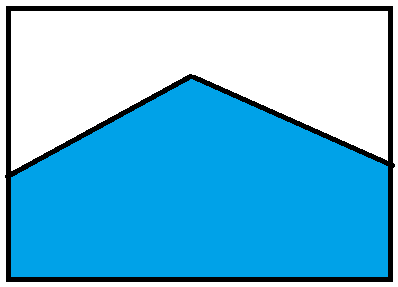
\includegraphics[width=\textwidth]{img/partial-table-invalid-case.png}
        \caption{위치 추정이 불가}
    \end{subfigure}
    \caption{당구대의 일부분만 시야에 들어오는 경우}
\end{figure}

임의의 position과 rotation으로 당구대의 모델을 화면에 투영하고, 투영된 컨투어 목록과 검출된 컨투어 목록 사이의 오차를 계산하여 반복적으로 오차를 줄여나가는 방법이다.

그러나 단순히 컨투어 목록을 OpenCV가 제공하는 projection method
\footnote{cv::projectPoints}
를 활용하면 일부 정점은 단순히 화면 밖으로 투영되고, \cref{fig;invalid-sight-projection}에서와 같이 화면의 경계선에 걸쳐 있는 점들과의 오차를 제대로 계산할 수 없다. 따라서 모델 정점들을 화면에 투사하기 전, 먼저 시야 범위를 구성하는 네 개의 평면에 맞춰 범위를 벗어나는 정점들에 대해 절단을 수행한다.

\begin{figure}[h]
    \centering
    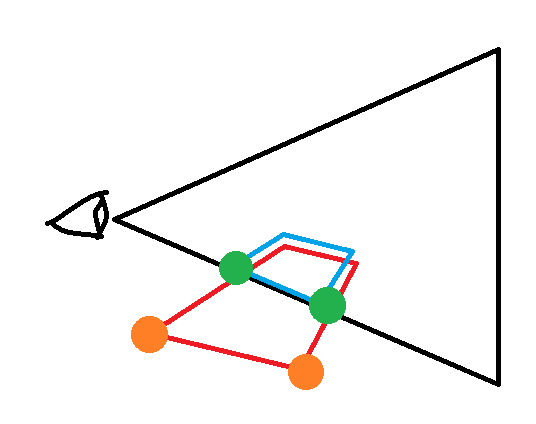
\includegraphics[width=7cm]{img/sight-invalid-culling.png}
    \caption{모델 정점을 그대로 화면에 투사할 시 일부 정점이 화면에서 이탈한다}
    \label{fig;invalid-sight-projection}
\end{figure}

위 과정을 거쳐 추정 위치 및 회전으로 투사된 정점 목록을 검출된 정점과 비교해 오차를 계산한다. 이 때  투사된 정점 목록의 인덱스를 시계 방향으로 한 번씩 회전시키며, 정점 사이의 거리(오차)의 합 $\sum_{n=0}^{N}|\vec{P}_{pn} - \vec{P}_{sn}|$이 최소치가 되는 트랜스폼을 선택한다.

이후 위와 마찬가지로 카메라에 대한 당구대의 상대 포즈를 월드 좌표로 변환한다.


\subsection{당구공 인식}

\begin{figure}[ht]
    \centering
    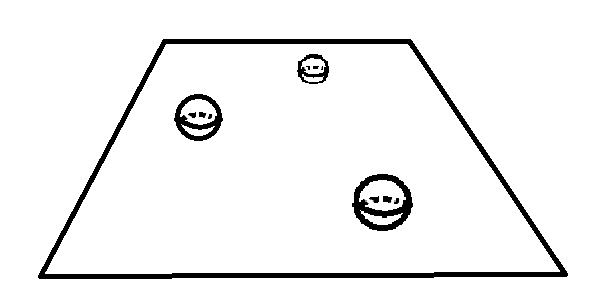
\includegraphics[width=8cm]{img/ball-recognition-introduce.png}
    \caption{당구공의 중점은 항상 한 평면상에 존재한다}
    \label{fig;ball-recognition-intro}
\end{figure}

당구공은 완전한 구의 형태이며, 따라서 카메라에서 2D 이미지 상 원형의 중점으로 광선(a)을 투사하면 반드시 구의 중점을 지나게 된다. 또, 구의 중점은 반드시 당구대 표면에서 일정한 거리로 떨어진 평면(b) 상에 존재한다.

이 과정은 \cref{fig;ball-recognition-howto}에 잘 나와있다.

\begin{figure}[ht]
    \centering
    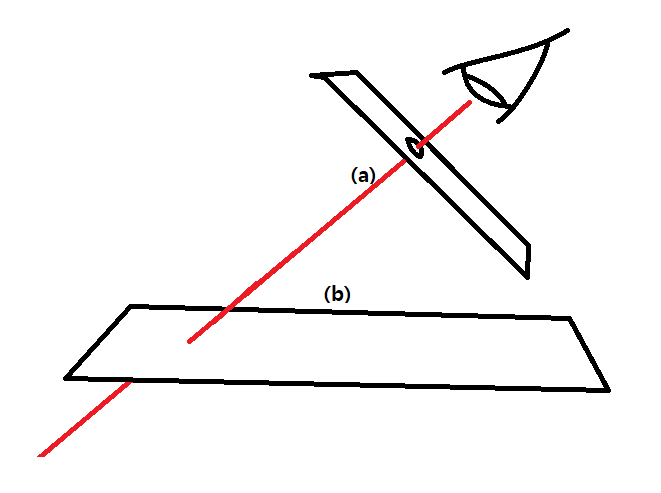
\includegraphics[width=8cm]{img/ball-recognition-howto.png}
    \caption{(b)는 당구공의 중점이 존재할 수 있는 평면이다}
    \label{fig;ball-recognition-howto}
\end{figure}

이미 위에서 당구대의 3D 포즈를 계산하였다. 이렇게 계산된 포즈는 당구대의 바깥쪽 쿠션 높이를 기준으로 한 평면이므로(\cref{fig;cushion-height-example}의 A), 평면 (b)는 당구대 평면을 노멀 반대 방향으로 약간 오프셋하여 손쉽게 계산할 수 있다.

\begin{figure}[ht]
    \centering
    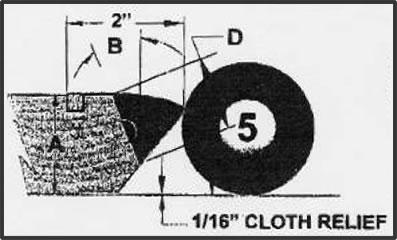
\includegraphics[width=8cm]{img/cushion-height-example.png}
    \caption[Caption for LOF]{당구대 쿠션 높이 예시\footnotemark}
    \label{fig;cushion-height-example}
\end{figure}
\footnotetext{이미지 출처: https://www.pooltablefeltcloth.com/cushion-height-guide-for-k-66-k-55.html}

다음으로 필요한 것은 각 공의 중점을 찾아내는 것이다. 탑-다운으로 이미지를 촬영해 이미지 상에서 공의 크기가 균일하고 공 사이에 폐색\textss{occlusion}이 발생하지 않는 일반적인 당구 보조 프로그램과 달리, AR 당구는 사용자 시점에서 영상 인식을 수행해야 하기 때문에 거리에 따라 구체의 이미지 상 반지름이 다르고, 폐색 또한 발생할 수 있다.

\begin{figure}
    \centering
    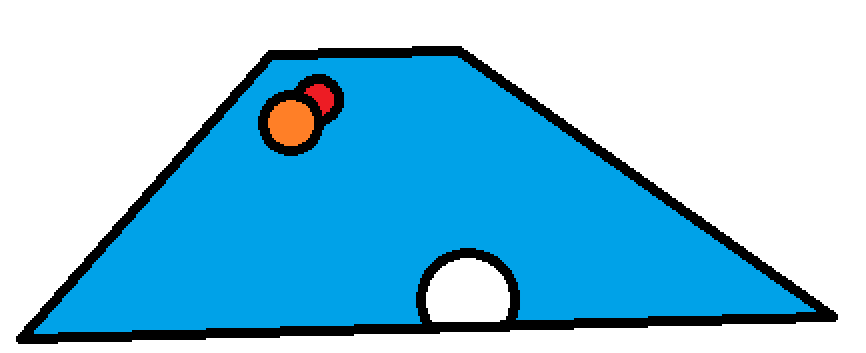
\includegraphics[width=8cm]{img/billiards-ar-view.png}
    \caption{AR 당구의 당구공 인식은 더 많은 요인을 고려해야 한다}
\end{figure}
카메라로부터의 거리에 따라 변화하는 공 원형의 반지름에 대응하기 위해 공을 검출하기 위한 커널의 크기를 매 평가시마다 동적으로 조절한다. 이 과정은 \cref{algo;kernel-radius}에 서술되어 있듯, 임의의 2D 점에 대한 먼 3D 점을 구하고, 카메라 원점 $(0, 0, 0)$과 해당 점 사이에 광선을 투사해 평면 (b)와 만나는 지점의 z 값을 찾음으로써 이루어진다.

\begin{algorithm}
    \caption{Estimate ball radius scale of given pixel coordinate}
    \label{algo;kernel-radius}
    \SetAlgoLined
    $\vec{P}_{ball} (u, v) \gets$ [Input] 2D point of estimated circle center \\
    $\vec{P}_{ray} (x, y, z) \gets$ $\vec{P}_{ball}$'s 3D coordinate assuming z as 10 \\
    $\vec{P}_{ball3} (x, y, z) \gets$ contact between $(0, 0, 0)$ and $\vec{P}_{ray}$ on the table plane (b) \\
    \KwResult{Evaluation kernel's radius scale is $z^{-1}$}
\end{algorithm}

\subsubsection{적합도 평가}
일반적으로, AR 당구의 사용자 시점에서 공은 다른 공에 의해 폐색될 수 있다. 즉, 많은 경우 공을 찾는 알고리즘은 오차가 적은 공보다 더 가능성이 높아 보이는 공을 찾게 된다. 이 과정을 직관적으로 수행하기 위해 각 중점 후보를 평가하는 과정에서 오차치가 아닌 적합도를 계산한다.

적합도는 오차 $\epsilon$에 대한 함수로, 적합도 $$a=\alpha^{-\epsilon^2}$$로 계산한다(\cref{fig;suitability-alpha-comparison}). 이 때 $\alpha$는 적합도의 허용치를 결정하는 계수로 여기서는 1.015로 두었다. 이 식에서 각 경우(픽셀 또는 정점의 비교, 후술)의 적합도 최대치는 오차가 0인 경우 1이다.

\begin{figure}[ht]
    \centering
    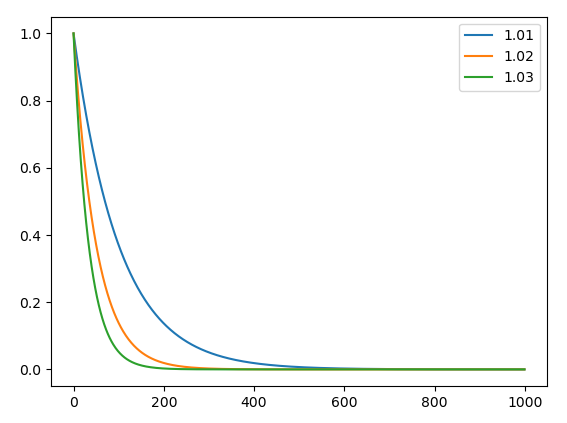
\includegraphics[width=7cm]{img/suitability-alpha-comparison.png}
    \caption{$\alpha$ 값에 따른 오차에 대한 적합도 그래프}
    \label{fig;suitability-alpha-comparison}
\end{figure}

\subsubsection{경계 적합도}
먼저 이미지의 HSV 색공간 표현에 대해 각 공 별로 필터링을 적용,



% ---------------------------------------------- REFERENCE SECTION
\end{comment}

\bibliographystyle{unsrt}
\bibliography{content.bib}

\end{document}
